% Created 2017-01-13 Fri 11:01
\documentclass[11pt]{article}
\usepackage[utf8]{inputenc}
\usepackage[T1]{fontenc}
\usepackage{fixltx2e}
\usepackage{graphicx}
\usepackage{longtable}
\usepackage{float}
\usepackage{wrapfig}
\usepackage{rotating}
\usepackage[normalem]{ulem}
\usepackage{amsmath}
\usepackage{textcomp}
\usepackage{marvosym}
\usepackage{wasysym}
\usepackage{amssymb}
\usepackage{hyperref}
\tolerance=1000
\date{Jan 21, 2017}
\title{Week 1 lecture notes - PSYC 5301}
\hypersetup{
  pdfkeywords={},
  pdfsubject={},
  pdfcreator={Emacs 25.1.1 (Org mode 8.2.10)}}
\begin{document}

\maketitle


\section*{Philosophical underpinnings}
\label{sec-1}
The goal of research is to find the \textbf{one truth}\ldots{}however, the \textbf{paths are many}.  Let's see how an ancient Hindu text can actually serve as a metaphor for how we do science.

Three paths to enlightenment (Bhagavad Gita, 500 BCE):
\begin{enumerate}
\item Karma yoga - the path of \emph{action}
\item Jnana yoga - path of \emph{knowledge}
\item Bhakti yoga - path of \emph{devotion}
\end{enumerate}

These map nicely onto Royall's (1997) three questions one should ask regarding data:
\begin{enumerate}
\item What should I do?
\item What's the relative evidence?
\item What should I believe?
\end{enumerate}

Paths for research:
\begin{enumerate}
\item \textbf{Path of action}: search for rules to govern our \emph{behavior} such that, in the long run, we will not be wrong too often
\begin{itemize}
\item $p < \alpha$: reject $H_0$
\item $p > \alpha$: remain in doubt
\item A rule to govern our \emph{behavior} in the \emph{long run}.  It tells us \emph{nothing} about the \emph{current test}.
\end{itemize}

\item \textbf{Path of knowledge}:  compare the likelihood of different hypotheses, given the data.
\begin{itemize}
\item suppose you flip a coin 10 times: you get 6 heads and 4 tails.  Is the coin biased (unfair)?
\item Two hypotheses: 
\begin{itemize}
\item $H_1$: the coin is biased (the true proportion of heads/tails is 0.6
\item $H_2$: the coin is fair (true proportion of heads/tails is 0.5
\item Question: given the data, how much more likely is $H_1$ than $H_2$
\item 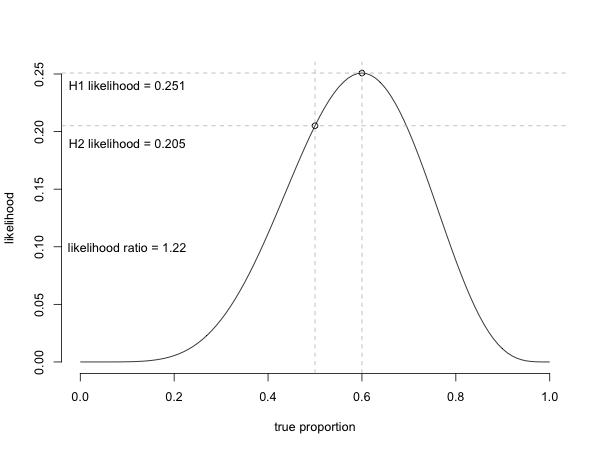
\includegraphics[width=.9\linewidth]{figures/coinFlip.png}
\end{itemize}
\end{itemize}

\item \textbf{Path of belief}: do I really \emph{believe} this coin will come up heads 60\% of the time?
\begin{itemize}
\item No\ldots{}I have \emph{prior} beliefs.
\item One "experiment" with 6 heads does not \emph{change} my prior beliefs
\end{itemize}
\end{enumerate}


These paths form the basis of three dominant statistical paradigms in the psychological literature:
\begin{enumerate}
\item Neyman-Pearson (the most common)
\item Likelihood
\item Bayesian
\end{enumerate}

\subsection*{Neyman-Pearson method}
\label{sec-1-1}

Historically, our method of hypothesis testing (using $p$-values) is an amalgamation of two (quite different) ideas from a couple of early 20th century statisticians:

\begin{itemize}
\item Jerzy Neyman: $p$-value tells you what \emph{action} to perform.  If $p<\alpha$, then we reject null hypothesis
\item Ronald Fisher: $p$-value measures evidence\ldots{}the smaller the $p$-value, the greater the evidence (this is actually incorrect)
\item Note: when I teach undergraduate statistics, I teach \emph{only} the Neyman method.  - define $H_0$
\begin{itemize}
\item set $\alpha$ (usually 0.05) and find the critical test statistic
\item if test statistic exceeds critical, we we reject $H_0$ (action)
\end{itemize}
\item However, most psychological literature (and many courses) implicitly tack on the incorrect Fisher ideas.  
\begin{itemize}
\item Example: I got $p=0.03$ for "Effect 1" and $p=0.003$ for "Effect 2"..which has "more evidence"?
\item Answer: neither, but Fisher thought Effect 2 would have more evidence
\item this understanding is implicit everywhere in psychology, but it is wrong!
\end{itemize}
\end{itemize}
This is why we hyphenate the two and refer to the entire paradigm as "Neyman-Fisher"
% Emacs 25.1.1 (Org mode 8.2.10)
\end{document}